% Finalizado
\chapter{Mejoras respecto al código inicial}

Durante el desarrollo no solo creamos las partículas. También optimizamos y limpiamos el código base del motor. Estas mejoras hacen que la aplicación sea más sólida, facilitan la programación y mejoran la usabilidad. Detallamos los cambios principales a continuación.

\section{Punteros inteligentes}
Refactorizamos el motor a fondo. Eliminamos los viejos punteros crudos (\textit{raw pointers}) de C y los cambiamos por punteros inteligentes (\textit{smart pointers}) de C++ moderno. Esta estrategia afecta a todas las clases. Buscamos asegurar la gestión de la memoria. Queremos evitar a toda costa las fugas de recursos (\textit{memory leaks}).

Para lograrlo, usamos dos herramientas clave:
\begin{itemize}
    \item \textbf{Uso de \texttt{std::unique\_ptr}:} Indica propiedad exclusiva. Las piezas geométricas (\texttt{GEPiece}) de un objeto 3D pertenecen solo a ese objeto. Si destruimos la entidad padre, el puntero inteligente libera su memoria en el acto. Seguimos el paradigma RAII.
    \item \textbf{Uso de \texttt{std::shared\_ptr}:} Lo reservamos para recursos compartidos. Es el caso de las texturas (\texttt{GETexture}). Así, decenas de modelos distintos apuntan a la misma textura en VRAM de forma segura. El recurso solo se borra cuando nadie más lo usa. El contador llega a cero y se libera.
\end{itemize}

\section{Capa de Validación de Vulkan}
Vulkan busca el rendimiento bruto. Por eso, no comprueba si el desarrollador comete errores en tiempo de ejecución. Delega todo el control de la memoria. Para no programar a ciegas, activamos la capa de validación oficial (\textit{Vulkan Validation Layer}). Este sistema actúa como un filtro entre nuestro código y el controlador gráfico. Analiza cada llamada de la API. Como muestra la Figura~\ref{fig:codigoValidacion}, inyectamos la capa de Khronos al arrancar la instancia. El entorno revisa la sincronización y los parámetros en directo, enviando alertas claras a la consola ante cualquier fallo \parencite{vulkan_validation}.

\begin{figure}[ht]
    \centering
\begin{carbonbox}
const char* validationLayers[] = { "VK_LAYER_KHRONOS_validation" };

createInfo.enabledLayerCount = 1;
createInfo.ppEnabledLayerNames = validationLayers;
\end{carbonbox}
    \caption{Activación de la capa de validación de Khronos en la creación de la instancia.}
    \label{fig:codigoValidacion}
\end{figure}

\section{TinyObjLoader}
Queríamos montar escenas más ricas. Por eso, integramos la librería externa \texttt{tinyobjloader} \parencite{tinyobjloader}. Es un analizador (\textit{parser}) de C++ muy ligero. Nos sirve para leer archivos 3D en formato Wavefront OBJ. La librería agiliza la lectura de vértices, normales y mapas UV. Así metemos mallas complejas en la GPU sin complicaciones.

\subsection{Adaptación estructural: \texttt{GEObject} y \texttt{GEModel}}
El soporte de mallas complejas nos obligó a cambiar la estructura. Modificamos la clase base \texttt{GEObject} y creamos \texttt{GEModel}.

Convertimos la clase abstracta \texttt{GEObject} en un contenedor genérico y seguro. Ahora guarda vectores de punteros inteligentes para sus texturas (\texttt{std::shared\_ptr<GETexture>}) y sus piezas (\texttt{std::unique\_ptr<GEPiece>}). Gracias a este cambio, un solo objeto puede tener sub-mallas con materiales distintos. Centralizamos el dibujo, las matrices de modelo y los cambios en un único sitio.

A partir de ahí programamos \texttt{GEModel}. Esta clase hereda de \texttt{GEObject} y exprime las funciones de \texttt{tinyobjloader}. El proceso de carga tiene cuatro pasos:
\begin{enumerate}
    \item \textbf{Lectura del archivo:} Con \texttt{tinyobj::LoadObj} leemos los ficheros \texttt{.obj} y \texttt{.mtl}. El motor busca las rutas de las imágenes en el disco de forma dinámica.
    \item \textbf{Control de fallos:} Cargamos los archivos en la VRAM. Para evitar cuelgues (\textit{crashes}) si falta un archivo, usamos un bloque \texttt{try-catch}. Si algo falla, el motor asigna una textura por defecto y la ejecución sigue.
    \item \textbf{Limpieza de duplicados:} Los archivos OBJ repiten vértices para armar las caras del objeto. Para no tirar memoria en la GPU, creamos una tabla hash (\texttt{std::unordered\_map}) a medida para \texttt{GEVertex}. Cruzamos posiciones, normales y UVs para borrar repetidos y optimizar el búfer de índices.
    \item \textbf{Montaje:} Creamos un \texttt{GEPiece} por cada sub-malla (\textit{shape}). Le metemos los búferes optimizados y su textura. Al final, transferimos la propiedad de las piezas al modelo usando semántica de movimiento (\texttt{std::move}). Cero copias innecesarias.
\end{enumerate}

\section{Modos de cámara}
Inspeccionar las partículas en detalle requería mejores controles. Por este motivo, rediseñamos la cámara. Añadimos dos modos nuevos (FPS y orbital) al modo libre que ya venía en el código base. El usuario cambia de modo pulsando el teclado. Los cálculos internos usan matrices de proyección y rotación estándar \parencite{lengyel2011mathematics}.

Implementamos estas tres opciones:
\begin{itemize}
    \item \textbf{Modo Libre:} Es el original. Permite volar por la escena sin límites.
    \item \textbf{Modo FPS:} Se mueve de forma similar a un juego en primera persona.
    \item \textbf{Modo Orbital:} Bloquea el objetivo en el centro del emisor que elijas. Puedes girar alrededor, hacer zoom y saltar de un sistema a otro de forma suave.
\end{itemize}

\section{ImGui}
Para vigilar el rendimiento del motor en tiempo real, metimos la interfaz \textit{Dear ImGui} \parencite{dearimgui}. Trabaja bajo el paradigma de modo inmediato (\textit{Immediate Mode GUI}). Su impacto en la CPU es mínimo. Dibujamos un panel transparente (\textit{overlay}) que muestra datos vitales: fotogramas por segundo (FPS), partículas vivas, tipo de cámara y controles. Nos ayuda a detectar fallos rápido.

\begin{figure}[ht]
    \centering
    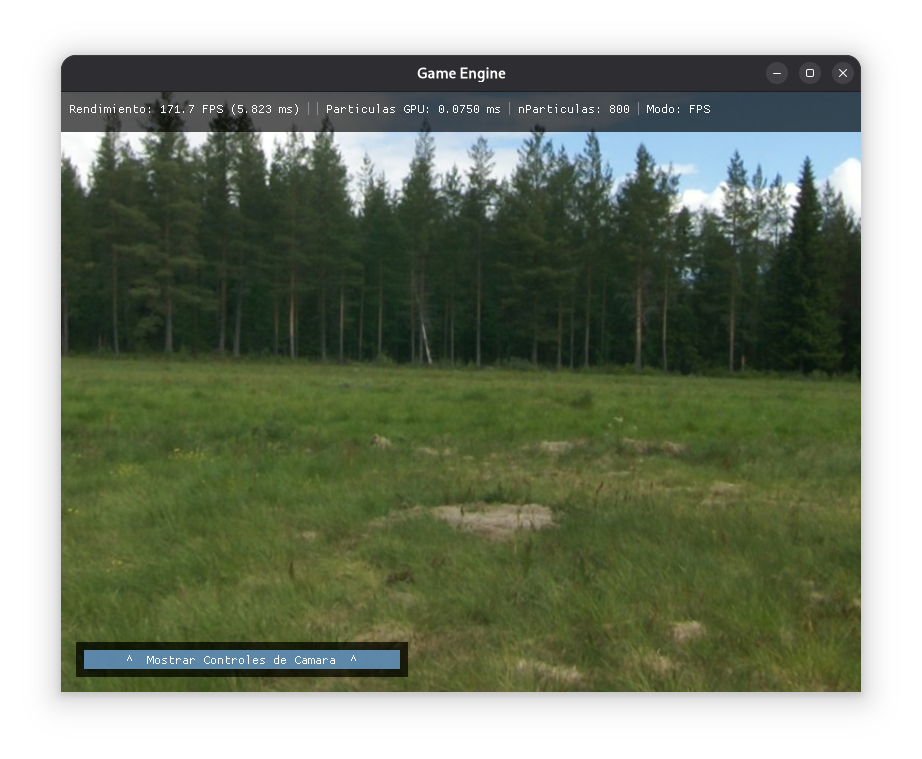
\includegraphics[width=1\textwidth]{Media/MejorasRespectoAlCodigoBase_1.png}
    \caption{Interfaz de la aplicación.}
    \label{fig:ImGui}
\end{figure}

Buscamos un diseño limpio, como se ve en la Figura~\ref{fig:ImGui}. No queríamos tapar la simulación. Arriba del panel va la telemetría general: fotogramas, milisegundos por frame y total de partículas en ejecución. Abajo a la izquierda dejamos una lista con los atajos de teclado de la cámara activa. Sirve de chuleta para el usuario.

\subsection{Adaptación estructural e integración en Vulkan}
Pintar una interfaz de modo inmediato en una API tan directa como Vulkan es un reto. Hay que sincronizar los recursos de forma óptima o el rendimiento en fotogramas por segundo caerá drásticamente.

Integrar esta funcionalidad alteró significativamente el diseño arquitectónico inicial del motor. Originalmente, la aplicación grababa todas las instrucciones de renderizado de forma monolítica mediante la función \texttt{fillCommandBuffer}. Debido a los requisitos de actualización por cuadro de ImGui, dicha estructura fue descartada y fragmentada en métodos modulares repartidos entre los contextos correspondientes (\texttt{GECommandContext} y \texttt{GEGraphicsContext}) y los gestores de la propia interfaz gráfica.

El ciclo de vida y la grabación de comandos de la interfaz en el motor se estructuran en cuatro fases fundamentales:

\begin{enumerate}
    \item \textbf{Reserva de espacio e inicialización:} Vulkan exige conocer de antemano los recursos que utilizará la interfaz. Como se detalla en la Figura~\ref{fig:imgui_init}, se reserva un pool de descriptores (\texttt{VkDescriptorPool}) exclusivo para los muestreadores (\textit{samplers}) de ImGui. Posteriormente, se inicializa el sistema vinculando la ventana gestionada por GLFW y el contexto de Vulkan.

\begin{figure}[ht]
    \centering
\begin{carbonbox}
void GEApplication::inicializarImGui() {
    VkDescriptorPoolSize pool_sizes[] = {{ VK_DESCRIPTOR_TYPE_COMBINED_IMAGE_SAMPLER, 1 }};
    VkDescriptorPoolCreateInfo pool_info = {.sType = VK_STRUCTURE_TYPE_DESCRIPTOR_POOL_CREATE_INFO, .flags = VK_DESCRIPTOR_POOL_CREATE_FREE_DESCRIPTOR_SET_BIT, .maxSets = 1000, .poolSizeCount = 1, .pPoolSizes = pool_sizes};
    vkCreateDescriptorPool(gc->device, &pool_info, nullptr, &this->imguiPool);
    ImGui_ImplGlfw_InitForVulkan(this->window.get(), true);
    // ... Configurar init_info con Device, Queue, RenderPass e ImageCount ...
    ImGui_ImplVulkan_Init(&init_info);
}
\end{carbonbox}
    \caption{Inicialización del contexto de Dear ImGui y configuración del Descriptor Pool en Vulkan.}
    \label{fig:imgui_init}
\end{figure}

    \item \textbf{Puesta al día (\textit{New Frame}) y Maquetación:} Al comienzo de cada iteración del bucle principal (método \texttt{draw}), se prepara la interfaz capturando los eventos de periféricos y actualizando los temporizadores internos. Si el usuario interactúa haciendo clic sobre el panel, los eventos del ratón se detienen de forma prioritaria en la UI, impidiendo que la cámara rote por error. En esta etapa se definen los elementos que se pintarán en la barra superior flotante y se invoca la lógica de las ventanas secundarias (Figura~\ref{fig:imgui_draw}).

\begin{figure}[ht]
    \centering
\begin{carbonbox}
void GEApplication::draw(double fixedDt, int physicsSteps, double alpha, double frameTime) {
    ImGui_ImplVulkan_NewFrame();
    ImGui_ImplGlfw_NewFrame();
    ImGui::NewFrame();
    ControlsGUI(scene->getCamera());
    ImGui::Render();
    ImGui_ImplVulkan_RenderDrawData(ImGui::GetDrawData(), cb);
}
\end{carbonbox}
    \caption{Ciclo de actualización, maquetación e inserción de comandos de la interfaz gráfica por fotograma.}
    \label{fig:imgui_draw}
\end{figure}

    \item \textbf{Lectura de datos y renderizado dinámico:} Para mantener una separación clara entre los datos puros del motor y la presentación visual, se implementaron métodos como \texttt{ControlsGUI} (Figura~\ref{fig:imgui_controles}). Utilizando las directivas de modo inmediato de la librería, el panel evalúa el estado del objeto \texttt{GECamera} y modifica los textos informativos en tiempo real, sirviendo de guía contextual para el usuario.

\begin{figure}[ht]
    \centering
\begin{carbonbox}
void GEApplication::ControlsGUI(GECamera* cam) {
    ImGui::Begin("Controles de Camara", nullptr, flags);
    if (mostrarControles) {
        if (cam->getCurrentMode() == GECamera::CameraMode::FREE) {
            ImGui::TextColored(ImVec4(0.2f, 1.0f, 0.2f, 1.0f), "LIBRE (Normal)");
            ImGui::Text("M: Cambiar modo | Flechas: Rotar...");
        }
    }
    ImGui::End();
}
\end{carbonbox}
    \caption{Maquetación condicional del menú de controles en función del estado de la cámara del motor.}
    \label{fig:imgui_controles}
\end{figure}

    \item \textbf{Inyección en el Render Pass:} La interfaz debe dibujarse siempre en último lugar para garantizar que actúe como un \textit{overlay} plano sobre los objetos tridimensionales y el sistema de partículas. Durante la grabación del búfer de comandos (\texttt{VkCommandBuffer}), la llamada nativa \texttt{ImGui\_ImplVulkan\_RenderDrawData} se inserta justo antes de dar por finalizado el pase de renderizado actual, enviando la geometría de los menús directamente a la GPU.
\end{enumerate}

\subsection{Elementos expuestos en la interfaz}
Con el objetivo de no saturar la simulación con logs de consola, la información recolectada por el motor se organizó conceptualmente en cuatro categorías lógicas dentro del panel superior y los menús flotantes:
\begin{itemize}
    \item \textbf{Rendimiento de renderizado:} Muestra de forma constante la tasa de FPS y los milisegundos ($ms$) empleados por la CPU en computar cada frame. Permite evaluar de inmediato el impacto del renderizado de las partículas.
    \item \textbf{Simulación física en GPU:} Expone el número total de partículas activas en la escena y calcula mediante marcas de tiempo el coste exacto en milisegundos que le toma al \textit{compute shader} resolver la física.
    \item \textbf{Estado de la cámara:} Detecta dinámicamente si el usuario navega en modo Libre, FPS u Orbital, alternando los textos de la interfaz para refrescar la lista de atajos correspondiente.
    \item \textbf{Datos orbitales:} Cuando se activa el modo de cámara orbital, la interfaz refleja explícitamente el nombre del emisor o del objeto geométrico que está actuando como centro de masas de la órbita actual.
\end{itemize}


\section{Vcpkg}
Para cerrar la arquitectura del proyecto, elegimos el gestor de paquetes \textit{vcpkg} \parencite{vcpkg_ms}. Administra las librerías de C y C++. En estos entornos, compilar herramientas de terceros (como GLFW, GLM, ImGui o TinyObjLoader) suele dar fallos de enlazado. Usar \textit{vcpkg} automatiza la descarga y compilación a través de CMake. Nos asegura un entorno de trabajo limpio, portátil y que compila a la primera.